\documentclass[../body.tex]{subfiles}
\begin{document}
\label{MetricsSection}
Оценка модели производилась на данных, размеченных вручную. В качестве данных взяты видео концертов на ресурсе \href{https://www.youtube.com/}{YouTube} общей длительностью 6 часов.

В качестве метрик использованы классические метрики для сегментации:

\begin{itemize}
	\item Intersection over union:
	\begin{equation}
		\text{IoU}(A, B) = \cfrac{|A \cap B|}{|A \cup B|}
	\end{equation}
	\item F1-score:
	\begin{equation}
		\text{f1}(A, B) = \cfrac{2|A \cap B|}{|A| + |B|}
	\end{equation}
\end{itemize}

Также использована метрика ROC\_AUC (зависимость доли правильно угаданных примеров позитивного класса от доли неверно угаданных примеров позитивного класса), так как тестовых данных не очень много, а задачу задача сведена к поточечной бинарной классификации.

Таблица с метриками (\ref{MetricsTable}) приведена ниже.

\begin{table}[H]
	\centering
	\begin{tabular}{|c|c|}
		\hline Метрика & Значение \\
		\hline
		IoU & 0.9025\\
		\hline
		f1 & 0.9453 \\
		\hline 
		ROC\_AUC & 0.8943\\
		\hline
	\end{tabular}
	\caption{Таблица с метриками.}\label{MetricsTable}
\end{table}

Графики сравнения масок и ROC-кривой приведены на рисунках (\ref{Mask_plot}) и (\ref{ROC_plot}).


\begin{figure}[H]
	\centering
	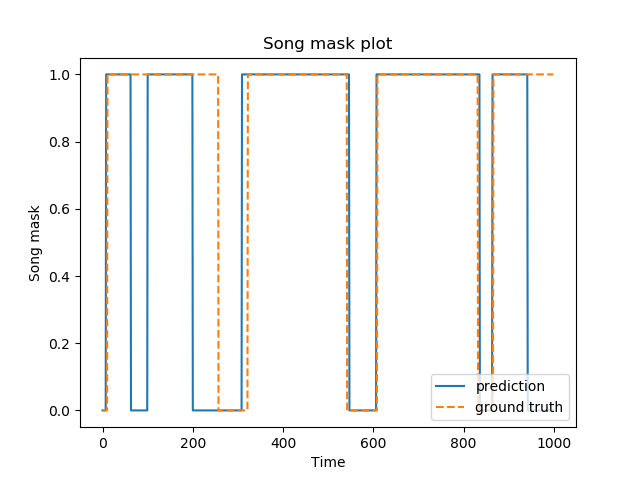
\includegraphics[scale=0.7]{images/masks.png}
	\caption{Сравнение масок}\label{Mask_plot}
\end{figure}

\begin{figure}[H]
	\centering
	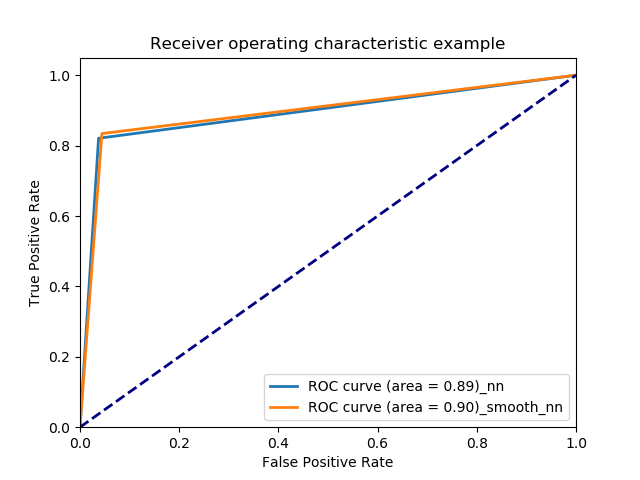
\includegraphics[scale=0.7]{images/roc_curve.png}
	\caption{ROC-кривая}\label{ROC_plot}
\end{figure}

\end{document}